\documentclass[10pt]{article}
\usepackage[margin=0.9in]{geometry}
\usepackage{amsmath,amssymb,amsthm,booktabs,array,hyperref,graphicx,microtype}
\hypersetup{colorlinks=true,linkcolor=blue,urlcolor=blue,citecolor=blue,pdftitle={Lean-Checked Travel Safety for a Sampled Actuator with Saturation}}
\newtheorem{theorem}{Theorem}
\newtheorem{proposition}{Proposition}
\newcommand{\R}{\mathbb R}
\newcommand{\E}{\mathcal E}
\newcommand{\clip}{\operatorname{clip}}
\newcommand{\norm}[1]{\left\lVert#1\right\rVert}
\newcommand{\code}[1]{\texttt{#1}}
\title{Lean-Checked Travel Safety for a Sampled Actuator with Saturation\\[3pt]
\large Exact certificates, sensor errors, and continuous execution}
\author{Mike\\\small Working draft; full author details and affiliation to be confirmed}
\date{17 October 2026}
\begin{document}
\maketitle
\begin{abstract}
We formalize a position-envelope guarantee for a sampled actuator with first-order lag, command saturation, timing jitter, and bounded held errors. Starting in an explicit full-state ellipsoid, every admitted execution remains within $|x(t)|\le2$ at every nonnegative real time, including between updates. The maximum normalized sampling interval is $1/5$, and the combined pre-clamp request-error and post-clamp disturbance budget is $1/100$. An admitted initial state requests twice the actuator limit, so the result includes genuine clipping. The Lean proof connects an exact exponential solution, four polynomial vertices, rational Bernstein matrix certificates, a step-scaled perturbation inequality, and a continuous assembled execution. Corollaries cover ideal sensor rounding and physical units. A response-bound ablation explains why a coarse estimate fails to certify the chosen budget; translated witnesses also replay in existing Lean SOS tooling. The contribution is a reproducible formal application and reusable proof composition. The control ingredients are established, and the result does not establish hardware safety or a verified finite-precision controller.
\end{abstract}

\section{Problem and contribution}
A sampled position controller can satisfy a discrete energy inequality without a theorem stating that position remains bounded between updates. Clipping, actuator dynamics, sensor error, and sampling jitter introduce further modeling obligations. We study a small axis model for which each obligation can be stated explicitly and joined in one Lean development. Our target is a symmetric position envelope about a fixed origin, not accumulated path length or a hard-stop contact model.

Let $z=(x,v,a)^\top$ and $k(z)=-x-3v-2a$. At sampling times $T_n=\sum_{j<n}h_j$, the controller chooses the command
\begin{equation}\label{eq:plant}
 u_n=\clip_{[-1,1]}(k(z_n)+e_n),\qquad
 \dot x=v,\quad \dot v=a,\quad \dot a=-a+u_n+d_n.
\end{equation}
The command, request error $e_n$, and disturbance $d_n$ are constant on each interval. The error $e_n$ enters before clipping; $d_n$ enters after clipping in the actuator command channel. Thus $|u_n|\le1$, while $|u_n+d_n|$ need not be at most one. The lag time constant and command limit are initially normalized. Section~\ref{sec:physical} gives a checked dimensional transformation.

The contribution has three parts. First, an explicit saturated execution has a checked all-time position bound, continuity across samples, and the stated ODE inside sampling intervals. Second, generic certificate, convexity, and perturbation interfaces connect untrusted rational witnesses to that execution; the request-error extension reuses the same certificate. Third, a reproducible artifact tests the model-to-certificate link, measures one source of conservatism, and translates the same vertex witnesses into an existing checker. We make no first-of-its-kind, optimal-controller, or comparative-speed claim. Related work already provides formal sampled control, verified control envelopes, and Lean positivity certificates; our proposed paper is a focused application case study.

\section{Safety contract and exact execution}
Define $\E(z)=z^\top Pz$ and the initial region $\mathcal S=\{z:\E(z)\le12\}$, where
\begin{equation}\label{eq:P}
 P=\begin{pmatrix}38/5&257/25&5\\257/25&1319/50&769/50\\5&769/50&278/25\end{pmatrix}.
\end{equation}
Positive energy bounds and rational positive-semidefinite witnesses establish
\begin{equation}\label{eq:geometry}
 x^2\le\E(z)/3,\qquad k(z)^2\le\E(z)/2,\qquad
 \E(z)\le M\norm{z}_2^2,\quad M=451/10.
\end{equation}
The set $\mathcal S$ restricts position, velocity, and acceleration jointly. It is not equivalent to the requested position interval.

For a constant drive $b=u+d$, the exact held solution from $z_0$ is
\begin{align}\label{eq:held}
 a(s)&=b+(a_0-b)e^{-s},\nonumber\\
 v(s)&=v_0+bs+(a_0-b)(1-e^{-s}),\\
 x(s)&=x_0+sv_0+bs^2/2+(a_0-b)(s-1+e^{-s}).\nonumber
\end{align}
The samples are defined recursively by evaluating this solution at $h_n$, using $b_n=\clip(k(z_n)+e_n)+d_n$. For $t\ge0$, the trajectory evaluates the same solution at $s=t-T_n$ in its unique containing half-open interval $[T_n,T_{n+1})$.

\begin{theorem}[Travel safety with measured requests]\label{thm:main}
Let $z_0\in\mathcal S$ and $h_{\min}>0$. For every sequence of durations and held errors satisfying
\[
 h_{\min}\le h_n\le1/5,\qquad |e_n|+|d_n|\le1/100\quad(n\in\mathbb N),
\]
the recursively defined execution of~\eqref{eq:plant} satisfies, for every real $t\ge0$,
\[
 \E(z(t))\le12,\qquad |x(t)|\le2.
\]
It agrees with the recursive samples, is continuous on $[0,\infty)$, and satisfies~\eqref{eq:plant} on every open sampling interval.
\end{theorem}
The minimum duration excludes infinitely many updates before a finite time: Lean proves $T_n\ge nh_{\min}$ and coverage and uniqueness of the containing interval. Matching endpoint identities join the analytic segments continuously. The ODE proof differentiates the exact solution and transfers it through the interval selector. We do not assert a derivative at switching times or uniqueness among all abstract ODE solutions. The theorem concerns the defined execution, whose continuity and interior dynamics are proved rather than assumed.

The result includes active clipping and nonzero errors. At $z_0=(0,0,1)^\top$, $\E(z_0)=278/25<12$. With $e_0=d_0=1/200$, the request is $-399/200<-1$ and the clipped command is $-1$. Lean also specializes the all-time theorem to this state, constant period $1/10$, and these constant nonzero errors. This establishes an admitted actively clipped initial condition; it does not assert perpetual saturation or that every sector extreme is attained.

\begin{proposition}[Position alone is insufficient]\label{prop:escape}
For the same controller, $z_0=(19/10,1,0)^\top$ has $|x_0|<2$ and command $-1$. With zero errors, its position at the admitted elapsed time $1/5$ exceeds $2$. This state has $\E(z_0)>12$.
\end{proposition}
The counterexample is checked in Lean using~\eqref{eq:held} and the exponential enclosure below. It illustrates why velocity and acceleration cannot be omitted from the initial condition, without contradicting Theorem~\ref{thm:main}.

\section{From the plant to rational certificates}
\subsection{Sector and exponential enclosure}
We first set $e=d=0$. For $z\in\mathcal S$,~\eqref{eq:geometry} implies a scalar sector representation
\[
 \clip(k(z))=\alpha k(z),\qquad 1/4\le\alpha\le1.
\]
The gain is selected from the sampled state and remains fixed over that held interval. Invariance re-establishes the sector condition at the next sample; it is not an independent global assumption about the trajectory.

Write $r=e^{-s}$ and
\[
 F_0(s,r)=\begin{pmatrix}1&s&s-1+r\\0&1&1-r\\0&0&r\end{pmatrix},\quad
 g(s,r)=\begin{pmatrix}s^2/2-s+1-r\\s-1+r\\1-r\end{pmatrix},\quad K=(1\;3\;2).
\]
The nominal held state is $A(s,\alpha,r)z=(F_0-\alpha gK)z$. Lean checks this identity against the analytic model, and proves
\begin{equation}\label{eq:enclose}
 1-s\le e^{-s}\le1-s+s^2\qquad(0\le s\le1).
\end{equation}
The matrix $A$ is affine in $r$ and in $\alpha$ separately. One shared exponential variable retains the dependence between coordinates. Four polynomial vertices, obtained at $\alpha\in\{1/4,1\}$ and $r\in\{1-s,1-s+s^2\}$, therefore suffice. The zero-elapsed-time case is handled separately, with no division by zero in the interpolation.

For a nonnegative quadratic form, Lean checks the identity
\[
 \E((1-\lambda)y+\lambda z)
 =(1-\lambda)\E(y)+\lambda\E(z)-\lambda(1-\lambda)\E(y-z).
\]
Applying it twice transfers a common vertex upper bound to every enclosed state. This step encloses the exact exponential solution; it does not replace that solution by a polynomial approximation without a remainder bound.

\subsection{Witness generation and checking}
For each polynomial vertex $A_j(s)$, an exact-rational Python producer constructs witnesses for
\begin{equation}\label{eq:cert}
 P-A_j(s)^\top P A_j(s)-sI=sR_j(s),\qquad R_j(s)\succeq0\quad(0\le s\le1/5).
\end{equation}
The matrix polynomial $R_j$ is expanded in a Bernstein basis on rational intervals. Each coefficient is supplied with an exact $LDL^\top$ factorization whose diagonal is nonnegative. Lean checks the reconstruction identities, diagonal inequalities, nonnegativity of the basis weights, and interval coverage. Positive lower and upper energy bounds are checked separately; decreasing a signed quadratic expression alone would not justify a bounded-state interpretation.

All four travel instances have cubic residuals, one interval $[0,1/5]$, and four Bernstein coefficient matrices. The producer is outside the proof trust boundary. Its output reports an unverified candidate until Lean checks it. Crucially, a valid certificate for a matrix supplied to the producer is insufficient: the handwritten model-to-vertex identities must connect that matrix to~\eqref{eq:held}. The resulting nominal statement is
\begin{equation}\label{eq:nominal}
 \E(A(s,\alpha,e^{-s})z)\le\E(z)-s\norm{z}_2^2.
\end{equation}
This is a decrease relative to the sampled state, not a claim that energy is monotone between every pair of intermediate times.

\section{Errors, sensing, and physical units}
\subsection{A perturbation bound that scales with elapsed time}
A held post-clamp error $w$ contributes exactly $g(s,e^{-s})w$. For $s>0$, dividing its two enclosure vertices by $s$ gives the affine vectors
\[
 (s/2,0,1)^\top,\qquad(-s/2,s,1-s)^\top.
\]
Their endpoint energies on $[0,1/5]$ are $278/25$, $3049/250$, and $7474/625$. Quadratic convexity and these exact values give
\begin{equation}\label{eq:response}
 \E(g(s,e^{-s})w)\le13s^2w^2.
\end{equation}
For $s>0$, apply the quadratic Young inequality with parameter $s\eta$, where $\eta=1/(2M)=5/451$. Combining~\eqref{eq:nominal}--\eqref{eq:response} yields
\begin{equation}\label{eq:step}
 \E(z(s))\le(1-s\eta)\E(z_n)+sD,\qquad
 D=13(1/5+1/\eta)(1/100)^2=1469/12500.
\end{equation}
Since $D<12\eta=60/451$ and $0\le s\eta\le1$, the region is invariant throughout each interval. The exact initial identity handles $s=0$. Scaling the Young parameter with $s$ avoids a fixed multiplicative energy penalty as elapsed time tends to zero. Induction at sample endpoints and clock coverage extend the segment result to every $t\ge0$.

For the actual measured request, define
\[
 w_{\mathrm{eff}}(z,e,d)=\clip(k(z)+e)-\clip(k(z))+d.
\]
Global nonexpansiveness of scalar clipping gives $|w_{\mathrm{eff}}|\le|e|+|d|$. Exact cancellation identifies the actual held segment with the nominal clipped segment driven by this effective error. Its sequence is computed from the already defined actual sample states, so no safe trajectory is assumed to construct it. This reduction proves Theorem~\ref{thm:main}, retaining active saturation and the same four certificates.

\subsection{Ideal sensor rounding}
For positive grid widths $\delta_x,\delta_v,\delta_a$, let $Q_\delta(y)=\delta\operatorname{round}(y/\delta)$ and use the request $-Q_{\delta_x}(x)-3Q_{\delta_v}(v)-2Q_{\delta_a}(a)$. Lean proves
\[
 |e_n|\le\delta_x/2+3\delta_v/2+\delta_a.
\]
A separate recursive execution computes these measurements from its own current sample state. Its all-time position bound follows if
\begin{equation}\label{eq:roundbudget}
 \delta_x/2+3\delta_v/2+\delta_a+W\le1/100,\qquad |d_n|\le W.
\end{equation}
For example, equal normalized grid widths $1/1000$ and $W=7/1000$ exhaust the budget. The initial state $(0,0,1)$ is represented exactly by these grids and still clips. This is ideal real-valued nearest-grid sensing; mathlib resolves half-integer ties toward positive infinity. It does not verify IEEE arithmetic, integer registers, overflow, or finite sensor range. The rounded corollary proves all-time safety and sample agreement; the separate measured-request execution has the explicit global continuity and interior-ODE theorems.

\subsection{A physical interpretation}\label{sec:physical}
For any known $\tau>0$ and acceleration-command limit $U>0$, define physical time and state by
\[
 t=T/\tau,\qquad z=(X/(U\tau^2),\ V/(U\tau),\ A/U)^\top.
\]
Lean proves the inverse transformations, sample-clock scaling, clipping homogeneity, and the actual physical dynamics
\begin{equation}\label{eq:physical}
 \dot X=V,\quad\dot V=A,\quad
 \dot A=\frac{-A+\clip_{[-U,U]}(q_n+\varepsilon_n)+\Delta_n}{\tau},\qquad
 q_n=-X_n/\tau^2-3V_n/\tau-2A_n.
\end{equation}
The rescaled measured execution is continuous, agrees with its samples, and satisfies~\eqref{eq:physical} inside each physical sampling interval. If
\[
 0<h_{\min}\le h_n\le\tau/5,\qquad
 |\varepsilon_n|+|\Delta_n|\le U/100,\qquad
 \E\bigl(X_0/(U\tau^2),V_0/(U\tau),A_0/U\bigr)\le12,
\]
then $|X(T)|\le2U\tau^2$ for every $T\ge0$. The physical errors are scalar request and drive errors in acceleration units. A physical grid-quantizer normalization theorem is not included.

\begin{center}
\begin{tabular}{ll}
\toprule
Illustrative assumption or consequence & Value\\\midrule
Known lag constant $\tau$; command limit $U$ & $0.1$ s; $2$ m/s$^2$\\
Maximum sample interval; combined error budget & $20$ ms; $0.02$ m/s$^2$\\
Certified displacement from origin & $|X(T)|\le 0.04$ m\\
Admitted initial state; initial requested/applied command & $(0,0,2)$; $-4/-2$ m/s$^2$\\\bottomrule
\end{tabular}
\end{center}
These constants are illustrative assumptions, not measurements from a robot. Changing $\tau$ changes both the plant and the prescribed controller gains; this parameterized family is not robustness to uncertainty in $\tau$.

\section{Evaluation and reproducibility}
\subsection{Which bound matters for this application?}
A coarse response estimate uses $\E(gw)\le M\norm{g}_2^2w^2$ and the same enclosure, giving $C=M(1+5H^2/4)=9471/200$ in place of $13$, with $H=1/5$. For the fixed region, error, and timing budget, the resulting sufficient condition fails:
\begin{center}
\begin{tabular}{lrrl}
\toprule
Response estimate & $C$ & $D=C(H+1/\eta)10^{-4}$ & Compare to $12\eta\approx0.13304$\\\midrule
Coarse norm bound & $47.355$ & $0.4280892$ & Fails this sufficient budget\\
Direct response energy & $13$ & $0.11752$ & Passes\\\bottomrule
\end{tabular}
\end{center}
Lean checks the two final rational comparisons. The coarse derivation is explanatory analysis; its failure does not prove that the plant is unsafe. The checked direct-energy bound is sufficient for the application. Neither the region, sampling limit, sector, nor error budget is claimed maximal. Proposition~\ref{prop:escape} separately provides an actual trajectory counterexample to a weakened initial condition.

\begin{figure}[tbp]
\centering
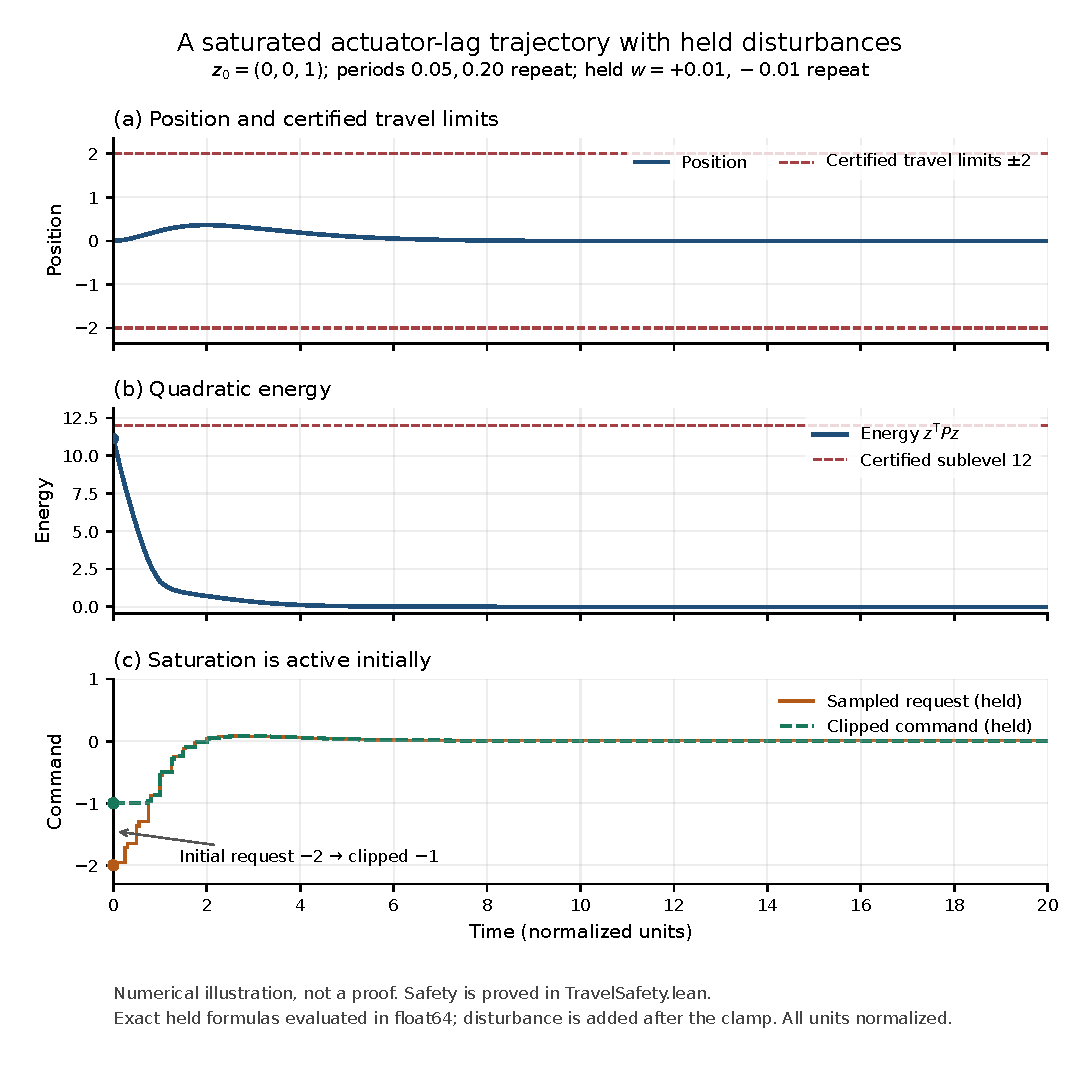
\includegraphics[width=0.76\textwidth]{images/travel-example.pdf}
\caption{Illustration from $(0,0,1)$ with alternating periods $1/20,1/5$, zero request error, and alternating held disturbances $1/100,-1/100$. Exact held formulas are evaluated in double precision. The observed excursion is much smaller than the certified envelope; this single trace does not measure worst-case conservatism. The Lean theorem, rather than this plot, covers every admitted sequence and every real time.}
\label{fig:travel}
\end{figure}

\subsection{Model binding and witness interoperability}
The verification workflow accepts the original saturated model, then changes the acceleration coefficient in $k(z)$ from $2$ to $3$ while preserving the generated certificate matrices. Lean rejects all four model-to-vertex identities. Additional producer tests accept a valid scalar certificate and reject a corrupt residual coefficient and a changed transition paired with its old witness. These tests exercise the intended rejection boundaries; they are not a substitute for the kernel proofs or an assessment of the modified controller's safety.

For a matched representation check, we translated the same four travel witnesses into 48 rational weighted squares and replayed them with upstream \code{sos\_witness}~\cite{sos}. All four residual nonnegativity proofs and their transition identities and decrease conclusions passed, with standard-axiom audits. The replay uses Lean 4.33.1 and SOS revision \code{fb7ae41}. Three fresh-process checks took 20.593, 9.049, and 9.260 seconds, with cached dependencies and a median of 9.260 seconds. These timings include imports and axiom queries, exclude discovery, and cover only the vertex statements. Different toolchains and theorem scopes prevent a speed comparison with the main development. This establishes shared-witness interoperability, not independent solver discovery or a second proof of the full saturated execution.

\subsection{Replay and claim map}
The main development pins Lean 4.35.0 and mathlib revision \code{56a0058}; full revisions, commands, input hashes, and logs are included in the artifact. Exact-rational production uses SymPy 1.14.0. The build checks a complete public theorem inventory and its transitive axiom closures against the allowlist \code{propext}, \code{Classical.choice}, and \code{Quot.sound}. No admitted proof or compiler-trust axiom is accepted. A fresh source-copy replay removes project build products while reusing the recorded pinned toolchain and isolated dependency caches. It is not a fresh bootstrap of Lean and all mathlib dependencies.

The fresh replay rebuilt all 43 project modules and audited 516 named public declarations in 52.61 seconds. It preserved all 83 frozen source/configuration files. The separate main workflow also passed producer, model-mutation, and benchmark-regeneration checks. These are single-machine measurements with the caching boundary described above.

The reusable layers are the Bernstein certificate interface, quadratic convexity, and elapsed-time-scaled robustness theorem. The four travel matrices and geometry witnesses are specific to this controller and region. The artifact retains earlier examples outside this paper; their existence is not evidence that the complete saturated guarantee generalizes to all those plants.

\begin{center}\small
\begin{tabular}{>{\raggedright\arraybackslash}p{0.35\textwidth}>{\raggedright\arraybackslash}p{0.57\textwidth}}
\toprule
Claim & Lean module and principal declaration\\\midrule
Exact held dynamics and four vertices & \code{SaturatedLag}: \code{heldSegment\_ode}, vertex identities\\
Held error response bound & \code{TravelDisturbance.response\_energy\_bound}\\
All-time base travel guarantee & \code{TravelSafety.travel\_limit}\\
Continuous base execution and ODE & \code{TravelExecution}: continuity, \code{state\_ode\_interior}\\
Measured execution calculus & \code{MeasuredTravel}: \code{state\_continuousOn\_nonnegative}, \code{state\_ode\_interior}\\
Request error and ideal sensing & \code{MeasuredTravel}: \code{travel\_limit}, \code{rounded\_travel\_limit}\\
Physical execution and envelope & \code{PhysicalTravel.measured\_travel\_limit}\\
Scope counterexample and ablation & \code{TravelScope}: \code{position\_only\_escapes}, budget comparisons\\\bottomrule
\end{tabular}
\end{center}
Successful checking establishes the formal statements relative to their definitions and permitted axioms. The Lean installation and imported dependency artifacts remain part of the software trust boundary. A theorem inventory count measures artifact coverage, not the number of new research results.

\section{Related work and limits}
Hellwig et al.~\cite{zonotope} connect numerical zonotope witnesses to KeYmaera X proofs of safe control envelopes, explicitly distinguishing one-step invariance, intersample safety, and control admissibility. Our work does not introduce that separation. It studies a fixed saturated feedback law, ellipsoidal energy witnesses, an exact lag solution, and a Lean execution with variable sampling intervals. The current evidence does not establish a general advantage over the zonotope pipeline. Earlier theorem-prover work already treats nondeterministic sampled closed-loop systems~\cite{closedloop}.

Doll and Shames~\cite{doll} develop machine-checked control foundations in Lean. Existing Lean SOS tooling checks rational positivity witnesses~\cite{sos}; MatrixSOS formalizes interval positivity for real symmetric univariate polynomial matrices~\cite{matrixsos}. Our Bernstein representation is a sufficient certificate construction, not a new positivity class. Sampled-data saturation and Lyapunov/sector methods also have established control-theoretic treatments, including magnitude and rate saturation~\cite{palmeira}. The present application includes magnitude saturation and a first-order lag, not a separately imposed rate limit.

The remaining assurance gap is concrete. No physical axis has been selected or calibrated. Friction, uncertain lag, computation and communication delay, unmodeled coupling, and within-interval disturbance variation are outside the plant. A real controller needs justified bounds for these effects and its arithmetic, or a stronger model. Ideal sensor rounding covers only one component. The theorem supplies a static invariant envelope; it does not implement a motion planner, runtime safety filter, or recovery policy from outside the ellipsoid. Human mathematical and application review, a clear reuse case, author details, and a release license remain prerequisites to submission.

\section{Conclusion}
The development connects exact saturated actuator dynamics to an all-real-time position envelope with timing jitter and a combined sensing/disturbance budget. The response-energy ablation shows a specific proof refinement that enables the chosen contract, and the shared-witness replay separates application composition from established positivity checking. The next useful extension is a second axis model with justified uncertainty or delay bounds, evaluated through the same interfaces. That would test reuse and practical relevance beyond this illustrative case.

\paragraph{Authorship and assistance.}
This is a local working draft for Mike. Full human author identity, affiliation, contributions, and acknowledgments require confirmation. AI assistance was used for exploration, proof implementation, writing, and review. The human author remains responsible for the mathematical claims, modeling choices, literature positioning, and final text. The draft has not been submitted or publicly released.

\begin{thebibliography}{9}\small
\bibitem{zonotope} J. Hellwig, L. Sch\"afer, L. Qian, A. Platzer, and M. Althoff. From Zonotopes to Proof Certificates: A Formal Pipeline for Safe Control Envelopes. \emph{iFM 2025}, LNCS 16194, 248--267, 2026. \url{https://doi.org/10.1007/978-3-032-10794-7_13}.
\bibitem{closedloop} N. Ar\'echiga et al. Using Theorem Provers to Guarantee Closed-Loop System Properties. \emph{American Control Conference}, 2012. \url{https://logic.kastel.kit.edu/ap/pub/TPgenloop.pdf}.
\bibitem{doll} M. Doll and I. Shames. Foundations of Machine-Checked Control Theory in Lean. 2026. \url{https://arxiv.org/abs/2607.19727}.
\bibitem{sos} Lean SOS contributors. SOS certificate tooling. Revision \code{fb7ae417609093f04cf0608dc92e9343550c2ae4}, inspected 17 October 2026. \url{https://github.com/leanprover/sos}.
\bibitem{matrixsos} M. Go. \emph{lean-matrix-sos}. Revision \code{02cfe73}, inspected 17 October 2026. \url{https://github.com/selpoG/lean-matrix-sos}.
\bibitem{palmeira} A. H. K. Palmeira, J. M. Gomes da Silva Jr., S. Tarbouriech, and I. M. F. Ghiggi. Sampled-data control under magnitude and rate saturating actuators. \emph{International Journal of Robust and Nonlinear Control} 26 (2016), 3232--3252. \url{https://doi.org/10.1002/rnc.3503}.
\end{thebibliography}
\end{document}
